

  
  
  
  
  
  
\documentclass[a4paper,11pt]{book}

\usepackage{marginnote}
\usepackage[left=2.1cm,top=2.4cm,right=2.1cm,bottom=2.2cm,marginparwidth=1.2cm]{geometry}
\usepackage{amsmath}
\usepackage[utf8]{inputenc}
\usepackage{graphicx}
\usepackage[T1]{fontenc}
% Index
\usepackage{imakeidx}
\makeatletter
\def\@idxitem{\par\hangindent 0pt}
\makeatother
\usepackage{filecontents}
\begin{filecontents}{\jobname.mst}
    heading_prefix "{\\bfseries\\hfil "
    heading_suffix "\\hfil}\\nopagebreak\n"
    headings_flag 1
    symhead_positive ""
    numhead_positive ""
    delim_0 "\\dotfill"
    delim_1 "\\dotfill"
    delim_2 "\\dotfill"
\end{filecontents}
%
\usepackage{latexsym}
\usepackage{fancyhdr}

\pagestyle{fancy}
\fancyhf{}
\renewcommand{\headrulewidth}{0pt}
\fancyfoot[C]{\thepage}

% added by CB 01/2020
\renewcommand{\sfdefault}{phv}
\renewcommand{\familydefault}{\sfdefault}
%\makeatletter
%\renewcommand{\@seccntformat}[1]{}
%\makeatother
\usepackage{titlesec,xcolor}
\definecolor{sitecolor}{HTML}{c95c50}
\titleformat{\section}[block]{\color{sitecolor}\Large\bfseries\filcenter}{}{1em}{}
\def\doubleline{
\hrule width \hsize height 0.5pt  \kern 1mm \hrule width \hsize height 0.5pt 
}
\setcounter{secnumdepth}{0} % sections are level 1
\usepackage[backref, pagebackref=false, hyperindex=true, breaklinks=true, colorlinks=true, urlcolor=magenta, linkcolor=sitecolor, citecolor=NavyBlue, citebordercolor={0 1 0}, pagecolor=red, bookmarks=true, filecolor=blue,bookmarksopen=true, plainpages=false, pdfpagemode=UseThumbs,linktocpage=true]{hyperref}
\usepackage{pdflscape} % schedule displayed in landscape format

%-----------------

% We will need to build up the authors index at the end of the booklet
\makeindex[program=makeindex,columns=3,intoc=true,title=Authors index]

\begin{document}
\frontmatter

\thispagestyle{empty}
\begin{titlepage}
  \centering
  
\includegraphics[width=.99\textwidth]{images/CS21baniere.jpg}
  \vspace{\stretch{1}}
  \par{\Huge 21st Cambridge Workshop: Cool Stars,\\ Stellar Systems and the Sun \par}
  \vspace{\stretch{0.5}}
  \par{\LARGE 22 - 26 June 2020\\  Toulouse, France \par}
  \vspace{\stretch{1}}
  \par{\Huge\bfseries Abstracts\par}
  \vspace{5cm}
  \newpage
  \thispagestyle{empty}
  \vspace*{\fill}
  % Bottom of the page
  {\large Last updated: \today\par}
\end{titlepage}

\thispagestyle{empty}
\tableofcontents

% Include notes on internet connection at conference:
\newpage
\addcontentsline{toc}{chapter}{Connection to Internet}

\par\noindent{\huge {\bf Connection to Internet}}
\\
\\
\par\noindent TBD (Eduroam etc.)
% Include foreword from the SOC chair:
\newpage
\addcontentsline{toc}{chapter}{Foreword}

\par\noindent{\huge {\bf Foreword}}
\\
\\
\par\noindent From the chair SOC
% Include code of conduct:
\newpage
\addcontentsline{toc}{chapter}{Code of Conduct \& Contact Information}

\par\noindent{\huge {\bf Code of Conduct \& Contact Information}}
\\
\\
\par\noindent Something similar to CS20?
% Include maps of the convention centre:
\newpage
\addcontentsline{toc}{chapter}{Maps}

\par\noindent{\huge {\bf Maps}}
\\
\\
\par\noindent Include local maps of Convention Centre etc.
% Include conference schedule:
\newpage
\addcontentsline{toc}{chapter}{Conference Schedule}

\begin{landscape}
\par\noindent{\huge {\bf Conference Schedule}}
\\
\\
\begin{center}
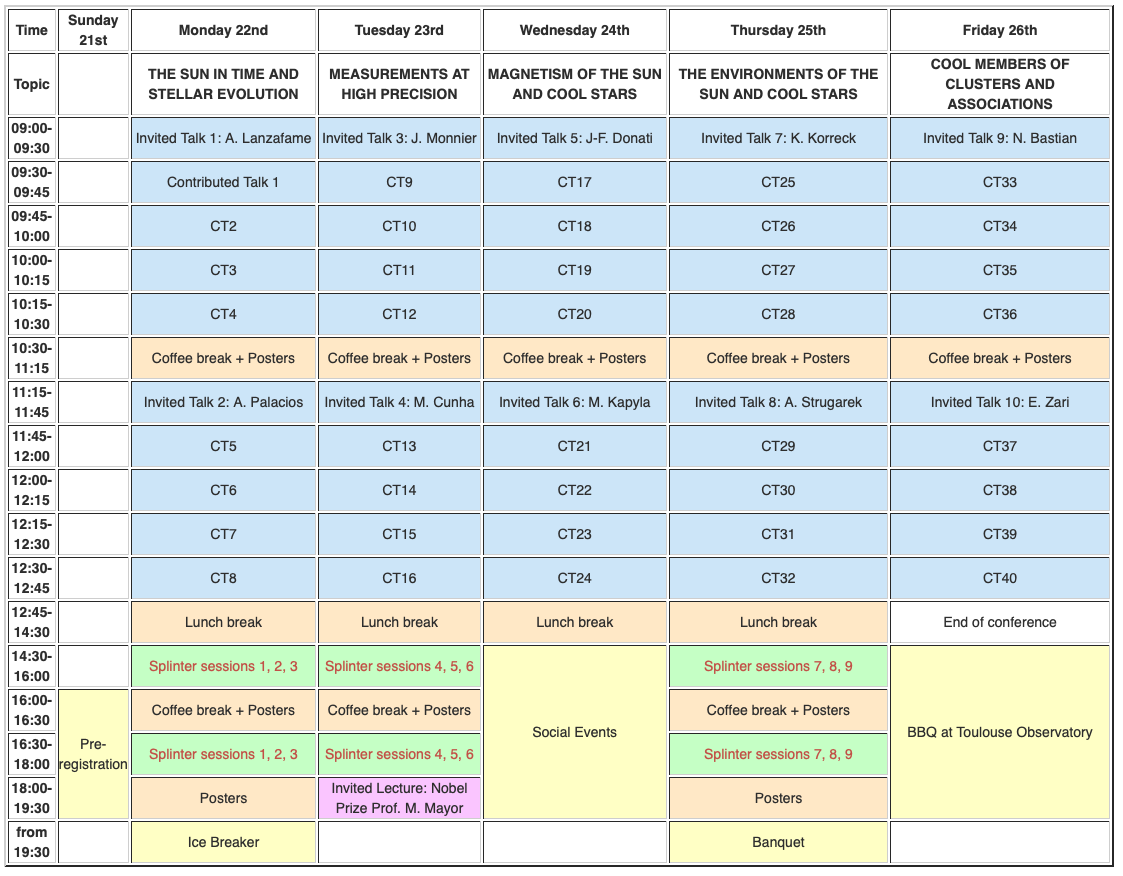
\includegraphics[width=1.15\textheight]{images/schedule.png}
\end{center}

\end{landscape}
% Include information on conference proceedings:
\newpage
\addcontentsline{toc}{chapter}{Instructions for the Conference Proceedings}

\par\noindent{\huge {\bf Instructions for the Conference Proceedings}}
\\
\\
\par\noindent TBD (Zenodo etc.)

\mainmatter


\chapter*{Talks}
\addcontentsline{toc}{chapter}{Talks}
        
          \section[Intermittent planet migration and the formation of multiple dust rings in protoplanetary disks \newline(Gaylor Wafflard-Fernandez)] { Intermittent planet migration and the formation of multiple dust rings in protoplanetary disks }



%%% ========================
%%% Display authors and their affiliation(s)
%%% ========================
\begin{center}
{\large Gaylor Wafflard-Fernandez};{ \large  Clément Baruteau}\\

%%% ===========================================
%%% Show schedule as a margin note for talks, or poster number for posters
%%% ===========================================


\marginnote{ TBA \\ TBA \\  }[0cm]



\index{"Wafflard-Fernandez" |textbf }\index{"Baruteau" } 
  
\vspace{2 mm}
\noindent IRAP, Université de Toulouse\\

\end{center}



%%% ===========
%%% Display abstract
%%% ===========
  
\vspace{2 mm}
\noindent An important challenge for understanding protoplanetary disks and planetary forma- tion is to be able to make a reliable connection between observed structures like bright and dark rings or asymmetries in radio emission observations provided by ALMA and the supposed presence of forming planets triggering these structures. Usually, the presence of N dark rings that are observed in real disks is interpreted as the presence of N fixed planets which would each create an accumulation of dust near the local maximum in the disk gas pressure. We show here that other configurations can explain these multiple rings. We use gas and dust hydrodynamical simulations with the 2D code FARGO to study the impact of the migration of a Saturn mass planet on the dust content of massive protoplanetary disks. When migration slows down, a pressure maximum forms beyond the plant that traps the large dust. We find a regime for which the planet migrates intermittently, with multiple runaway phases that lead to the formation of multiple sets of bright and dark rings beyond the planet’s location.

%%% separation with a double line
\noindent\doubleline
        
          \section[Dust traps in the protoplanetary disc MWC 758: two vortices produced by two giant planets? \newline(Clément Baruteau)] { Dust traps in the protoplanetary disc MWC 758: two vortices produced by two giant planets? }



%%% ========================
%%% Display authors and their affiliation(s)
%%% ========================
\begin{center}
{\large Clément Baruteau (1)};{ \large  Marcelo Barraza (2)};{ \large  Sebastián Pérez (3)};{ \large  Simon Casassus (4)};{ \large  Ruobing Dong (5)};{ \large  Wladimir Lyra (6)};{ \large  Sebastián Marino (7)};{ \large  Valentin Christiaens (8)};{ \large  Zhaohuan Zhu (9)};{ \large  Andrés Carmona (10)};{ \large  Florian Debras (11)};{ \large  Felipe Alarcon (12)}\\

%%% ===========================================
%%% Show schedule as a margin note for talks, or poster number for posters
%%% ===========================================


\marginnote{ TBA \\ TBA \\  }[0cm]



\index{"Baruteau" |textbf }\index{"Barraza" } \index{"Pérez" } \index{"Casassus" } \index{"Dong" } \index{"Lyra" } \index{"Marino" } \index{"Christiaens" } \index{"Zhu" } \index{"Carmona" } \index{"Debras" } \index{"Alarcon" } 
  
\vspace{2 mm}
\noindent (1) IRAP, Université de Toulouse; (2)  Universidad de Chile \& Max Planck Institute for Astronomy; (3)  Universidad de Chile; (4)  Universidad de Chile; (5)  University of Arizona; (6)  California State University Northridge \& Jet Propulsion Laboratory; (7)  Max Planck Institute for Astronomy; (8)  Universidad de Chile \& Monash Centre for Astrophysics; (9)  University of Nevada; (10)  IRAP, Université de Toulouse; (11)  IRAP, Université de Toulouse; (12)  Universidad de Chile\\

\end{center}



%%% ===========
%%% Display abstract
%%% ===========
  
\vspace{2 mm}
\noindent Resolved ALMA and VLA observations indicate the existence of two dust traps in the protoplanetary disc MWC 758. By means of 2D gas+dust hydrodynamical simulations post-processed with 3D dust radiative transfer calculations, we show that the spirals in scattered light, the eccentric, asymmetric ring and the crescent-shaped structure in the (sub)millimetre can all be caused by two giant planets: a 1.5-Jupiter mass planet at 35 au (inside the spirals) and a 5-Jupiter mass planet at 140 au (outside the spirals). The outer planet forms a dust-trapping vortex at the inner edge of its gap (at 85 au), and the continuum emission of this dust trap reproduces the ALMA and VLA observations well. The outer planet triggers several spiral arms which are similar to those observed in polarised scattered light. The inner planet also forms a vortex at the outer edge of its gap (at 50 au), but it decays faster than the vortex induced by the outer planet, as a result of the disc’s turbulent viscosity. The vortex decay can explain the eccentric inner ring seen with ALMA as well as the low signal and larger azimuthal spread of this dust trap in VLA observations. Finding the thermal and kinematic signatures of both giant planets could verify the proposed scenario.

%%% separation with a double line
\noindent\doubleline
        
          \section[Migrating super-Earths in low-viscosity discs: unveiling the roles of feedback, vortices, and laminar accretion flows \newline(Colin P. McNally)] { Migrating super-Earths in low-viscosity discs: unveiling the roles of feedback, vortices, and laminar accretion flows }



%%% ========================
%%% Display authors and their affiliation(s)
%%% ========================
\begin{center}
{\large Colin P. McNally (1)};{ \large  Richard P. Nelson (2)};{ \large  Sijme-Jan Paardekooper (3)};{ \large  Pablo Benítez-Llambay (4)}\\

%%% ===========================================
%%% Show schedule as a margin note for talks, or poster number for posters
%%% ===========================================


\marginnote{ TBA \\ TBA \\  }[0cm]



\index{"McNally" |textbf }\index{"Nelson" } \index{"Paardekooper" } \index{"Benítez-Llambay" } 
  
\vspace{2 mm}
\noindent (1) Queen Mary University of London; (2)  Queen Mary University of London; (3)  Queen Mary University of London \& University of Cambridge; (4)  Niels Bohr International Academy \\

\end{center}



%%% ===========
%%% Display abstract
%%% ===========
  
\vspace{2 mm}
\noindent We present the highest resolution study to date of super-Earths migrating in inviscid and low- viscosity discs, motivated by the connection to laminar, wind-driven models of protoplanetary discs. Our models unveil the critical role of vortices in determining the migration behaviour for partial gap-opening planets. Vortices form in pressure maxima at gap edges, and prevent the disc-feedback stopping of migration for intermediate planets in low-viscosity and inviscid discs, contrary to the concept of the ‘inertial limit’ or ‘disc feedback’ halting predicted from analytical models. Vortices may also form in the corotation region, and can dramatically modify migration behaviour through direct gravitational interaction with the planet. These features become apparent at high resolution, and for all but the highest viscosities there exist significant difficulties in obtaining numerically converged results. The migration of partial gap-opening planets, however, clearly becomes chaotic for sufficiently low viscosities. At moderate viscosity, a smooth disc-feedback regime is found in which migration can slow substantially, and the migration time-scale observed corresponds to migration being driven by diffusive relaxation of the gap edges. At high viscosity classical Type I migration is recovered. For Jupiter-analogue planets in inviscid discs, a wide, deep gap is formed. Transient Type II migration occurs over radial length-scales corresponding to the gap width, beyond which migration can stall. Finally, we examine the particle trapping driven by structures left in inviscid discs by a migrating planet, and find that particle traps in the form of multiple rings and vortices can persist long after the planet has passed. In this case, the observation of particle traps by submillimetre interferometers such as ALMA cannot be used to infer the current presence of an adjacent planet. 

%%% separation with a double line
\noindent\doubleline
        
          \section[Dispersal of protoplanetary disks by the combination of magnetically driven and photoevaporative winds \newline(M. Kunitomo)] { Dispersal of protoplanetary disks by the combination of magnetically driven and photoevaporative winds }



%%% ========================
%%% Display authors and their affiliation(s)
%%% ========================
\begin{center}
{\large M. Kunitomo}\\

%%% ===========================================
%%% Show schedule as a margin note for talks, or poster number for posters
%%% ===========================================


\marginnote{ TBA \\ TBA \\  }[0cm]



\index{"Kunitomo" |textbf }
  
\vspace{2 mm}
\noindent Kurume University, Japan\\

\end{center}



%%% ===========
%%% Display abstract
%%% ===========
  
\vspace{2 mm}
\noindent We investigate the roles of magnetically driven disk wind (MDW) and thermally driven photoevaporative wind (PEW) in the long-time evolution of protoplanetary disks. We start simulations from the early phase in which the disk mass is 0.118 Solar masses around a 1 $M_\star$ star and track the evolution until the disk is completely dispersed. We incorpo- rate the mass loss by PEW and the mass loss and magnetic braking (wind torque) by MDW, in addition to the viscous accretion, viscous heating, and stellar irradiation. We find that MDW and PEW respectively have different roles: magnetically driven wind ejects materials from an inner disk in the early phase, whereas photoevaporation has a dominant role in the late phase in the o 1 au) disk. The disk lifetime, which depends on the combination of MDW, PEW, and viscous accretion, shows a large variation of 120 Myr; the gas is dispersed mainly by the MDW and the PEW in the cases with a low viscosity and the lifetime is sensitive to the mass-loss rate and torque of the MDW, whereas the lifetime is insensitive to these parameters when the viscosity is high. Even in disks with very weak turbulence, the cooperation of MDW and PEW enables the disk dispersal within a few Myr.

%%% separation with a double line
\noindent\doubleline
        
          \section[Magnetic field of Betelgeuse during its supernova phase \newline(Pascal Petit)] { Magnetic field of Betelgeuse during its supernova phase }



%%% ========================
%%% Display authors and their affiliation(s)
%%% ========================
\begin{center}
{\large Pascal Petit (1)};{ \large  Tianqi Cang (2)};{ \large  Pierre Kervella (3)}\\

%%% ===========================================
%%% Show schedule as a margin note for talks, or poster number for posters
%%% ===========================================


\marginnote{ TBA \\ TBA \\  }[0cm]



\index{"Petit" |textbf }\index{"Cang" } \index{"Kervella" } 
  
\vspace{2 mm}
\noindent (1) IRAP, CNRS, Univ. Toulouse, CNES; (2)  IRAP, CNRS, Univ. Toulouse, CNES; (3)  LESIA, Observatoire de Paris\\

\end{center}



%%% ===========
%%% Display abstract
%%% ===========
  
\vspace{2 mm}
\noindent We measured the magnetic field of Betelgeuse during its supernova explosion. How cool is that?

%%% separation with a double line
\noindent\doubleline
        
          \section[La transhumance des truites \newline(Sébastien Deheuvels)] { La transhumance des truites }



%%% ========================
%%% Display authors and their affiliation(s)
%%% ========================
\begin{center}
{\large Sébastien Deheuvels };{ \large  Clément Baruteau}\\

%%% ===========================================
%%% Show schedule as a margin note for talks, or poster number for posters
%%% ===========================================


\marginnote{ TBA \\ TBA \\  }[0cm]



\index{"Deheuvels" |textbf }\index{"Baruteau" } 
  
\vspace{2 mm}
\noindent CNRS/Université de Toulouse\\

\end{center}



%%% ===========
%%% Display abstract
%%% ===========
  
\vspace{2 mm}
\noindent Abstract avec caractère latex comme $3\,M_{\odot}$

%%% separation with a double line
\noindent\doubleline
        
          \section[Effects of stellar winds on the perfomance of profesional basketball players \newline(Florian Debras)] { Effects of stellar winds on the perfomance of profesional basketball players }



%%% ========================
%%% Display authors and their affiliation(s)
%%% ========================
\begin{center}
{\large Florian Debras  (1)};{ \large  Michael Jordan (2)}\\

%%% ===========================================
%%% Show schedule as a margin note for talks, or poster number for posters
%%% ===========================================


\marginnote{ TBA \\ TBA \\  }[0cm]



\index{"Debras" |textbf }\index{"Jordan" } 
  
\vspace{2 mm}
\noindent (1) IRAP ; (2)  Chicago bulls\\

\end{center}



%%% ===========
%%% Display abstract
%%% ===========
  
\vspace{2 mm}
\noindent Within the past 10 years, there has been a decrease in the level of basketball players compare to the Michael Jordan era. Current studies have proposed, unconvicingly, to explain this trend by a change in food consumption or training practices. In this talk, we explore another possibility: an increase in thee stellar activity at the beginning of the 2010s. We first show that there are significant winds of dark matter originating from the sun, and treat the impact with basketball players brain using a machine learning approach. Finally, we will discuss the impact of non baryonic effects on the occurence rates of injuries, which has also drastically increased lately. All in all, we propose a simple, robust and observationnally favoured mecanism to explain the decrease in basketball skills in the past 20 years.

%%% separation with a double line
\noindent\doubleline
        
          \section[What can we learn from global MHD modeling of PSP encounters?  \newline(Victor Réville)] { What can we learn from global MHD modeling of PSP encounters?  }



%%% ========================
%%% Display authors and their affiliation(s)
%%% ========================
\begin{center}
{\large Victor Réville (1)};{ \large  Marco Velli (2)};{ \large  Anna Tenerani (3)};{ \large  Chen Shi (4)}\\

%%% ===========================================
%%% Show schedule as a margin note for talks, or poster number for posters
%%% ===========================================


\marginnote{ TBA \\ TBA \\  }[0cm]



\index{"Réville" |textbf }\index{"Velli" } \index{"Tenerani" } \index{"Shi" } 
  
\vspace{2 mm}
\noindent (1) IRAP/CNRS; (2)  University of California Los Angeles; (3)  University of Texas Austin; (4)  University of California Los Angeles\\

\end{center}



%%% ===========
%%% Display abstract
%%% ===========
  
\vspace{2 mm}
\noindent 
Global MHD models of the corona and solar wind are a key tool of the analysis of the Parker Solar Probe data. They can be used as a self-consistent framework to validate both the sources of the solar wind plasma measured in situ by PSP and a given theory of the solar wind birth and acceleration. Over the past decade, several Alfvén wave turbulence driven MHD models have been developed for this purpose with varying levels of complexity. We present here such a model which, using fairly simple assumptions on the wave energy propagation and dissipation, has shown to be able to reproduce most of PSP in situ large scale measurements. We show that in addition to the wind speed, density and magnetic field polarity, the amplitude of the perturbations is well recovered. This suggests that switchbacks, which have been observed to be a significant part of the magnetic field perturbations in the first PSP encounters, are fully part of the solar wind turbulence. Our model fails however to explain the peak tangential velocities observed close to the Sun, showing that some dynamics is missing. One possible explanation is the combined effect of the observed highly non linear Alfvénic switchbacks and pressure anisotropies on the angular momentum. We explore this hypothesis through analytical developments. 


%%% separation with a double line
\noindent\doubleline
        



\chapter*{Posters}
    \addcontentsline{toc}{chapter}{Posters}
        
          \section[A signature of planetary migration: the origin of the $2:1$ mean-motion resonance \newline(R. Murray-Clay)] { A signature of planetary migration: the origin of the $2:1$ mean-motion resonance }



%%% ========================
%%% Display authors and their affiliation(s)
%%% ========================
\begin{center}
{\large R. Murray-Clay for the UCSC team}\\

%%% ===========================================
%%% Show schedule as a margin note for talks, or poster number for posters
%%% ===========================================


\marginnote{ poster TBA }[0cm]



\index{"Murray-Clay" |textbf }
  
\vspace{2 mm}
\noindent University of California at Berkeley\\

\end{center}



%%% ===========
%%% Display abstract
%%% ===========
  
\vspace{2 mm}
\noindent The spatial distribution of Kuiper Belt objects (KBOs) in $2:1$ exterior resonance with Neptune constrains that planet’s migration history. Numerical simulations demonstrate that fast planetary migration generates a larger population of KBOs trailing rather than leading Neptune in orbital longitude. This asymmetry corresponds to a greater proportion of objects caught into asymmetric resonance such that their resonance angless librate about values greater than (trailing) as opposed to less than (leading). We provide, for the first time, an explanation of this phenomenon, using physical, analytic, and semianalytic arguments.

%%% separation with a double line
\noindent\doubleline
        
          \section[Cold dust emission from large-scale vortices induced by gap-opening planets \newline(Clément Baruteau)] { Cold dust emission from large-scale vortices induced by gap-opening planets }



%%% ========================
%%% Display authors and their affiliation(s)
%%% ========================
\begin{center}
{\large Clément Baruteau (1)};{ \large  Zhaohuan Zhu (2)};{ \large  Sebastian Pérez (3)};{ \large  Andrés Carmona (4)}\\

%%% ===========================================
%%% Show schedule as a margin note for talks, or poster number for posters
%%% ===========================================


\marginnote{ poster TBA }[0cm]



\index{"Baruteau" |textbf }\index{"Zhu" } \index{"Pérez" } \index{"Carmona" } 
  
\vspace{2 mm}
\noindent (1) IRAP, Université de Toulouse; (2)  University of Nevada, Las Vegas; (3)  Universidad de Chile; (4)  IPAG\\

\end{center}



%%% ===========
%%% Display abstract
%%% ===========
  
\vspace{2 mm}
\noindent High-resolution interferometric observations in the (sub)-mm have highlighted the presence of bright rings of dust emission in a number of protoplanetary discs. These emission rings are often lopsided, most notably in so-called transition discs. Despite limited observational evidence, these lopsided rings are so far best explained by dust trapping in a large-scale vortex in the gas. We investigate the observable consequences in the radio continuum of dust trapping in a vortex formed at the outer edge of the gap carved by a massive planet in its protoplanetary disc. From the spatial distribution of solid particles obtained in two-fluid 2D hydrodynamical simulations, we produce synthetic maps of the dust’s continuum emission at various wavelengths in the (sub)- mm. A range of disc masses is adopted to examine how gas self-gravity impacts the concentration and emission of solid particles trapped in the vortex. At large gas den- sities at the vortex’s radiaxl location (local background Toomre parameter is a few), gas self-gravity implies that several vortices form that merge and split intermittently. It makes the vortex long-lived and the dust emission forms a large-scale lopsided ring with possibly multiple peaks. Reducing the gas density leads to the formation of a single vortex with a much shorter lifetime. Before the vortex decays, the dust emission is confined to a rather narrow ring along which the flux contrast ratio is large. For moderate gas densities, the emission ring peaks at the vortex’s centre from sub-mm to mm wavelengths, and the azimuthal contrast ratio increases with wavelength. For small gas densities, the emission peak shifts from the vortex’s centre to about 90 de- grees ahead of the latter from sub-mm to mm wavelengths. As the vortex decays, solid particles lose their azimuthal trapping over different timescales depending on their size. This largely reduces the flux contrast ratio along the ring, which can decrease with wavelength.

%%% separation with a double line
\noindent\doubleline
        
          \section[The forming slow solar wind imaged along streamer rays by the wide-angle imager on Parker Solar Probe \newline(Nicolas Poirier)] { The forming slow solar wind imaged along streamer rays by the wide-angle imager on Parker Solar Probe }



%%% ========================
%%% Display authors and their affiliation(s)
%%% ========================
\begin{center}
{\large Nicolas Poirier (1)};{ \large Alexis P. Rouillard (2)};{ \large Athanasios Kouloumvakos (3)};{ \large Angelos Vourlidas (4)};{ \large Guillermo Stenborg (5)};{ \large Rui Pinto (6)}\\

%%% ===========================================
%%% Show schedule as a margin note for talks, or poster number for posters
%%% ===========================================


\marginnote{ poster TBA }[0cm]



\index{"Poirier" |textbf }\index{"Rouillard" } \index{"Kouloumvakos" } \index{"Vourlidas" } \index{"Stenborg" } \index{"Pinto" } 
  
\vspace{2 mm}
\noindent (1) IRAP, Université Toulouse III - Paul Sabatier, CNRS, CNES, Toulouse, France; (2) IRAP, Université Toulouse III - Paul Sabatier, CNRS, CNES, Toulouse, France; (3) IRAP, Université Toulouse III - Paul Sabatier, CNRS, CNES, Toulouse, France; (4) John Hopkins APL, Laurel, USA; (5) Naval Research Laboratory, Washington DC, USA; (6) IRAP, Université Toulouse III - Paul Sabatier, CNRS, CNES, Toulouse, France\\

\end{center}



%%% ===========
%%% Display abstract
%%% ===========
  
\vspace{2 mm}
\noindent The Wide-field Imager for Solar PRobe (WISPR) obtained the first high-resolution images of coronal rays at heights below 15 R$_\odot$ when Parker Solar Probe (PSP) was located inside 0.25 AU during the first encounter. We exploit these remarkable images to reveal the structure of coronal rays at scales that are not easily discernible in images taken from near 1 AU. To analyze and interpret WISPR observations which evolve rapidly both radially and longitudinally, we construct a latitude versus time map using full WISPR dataset from the first encounter. From the exploitation of this map and also from sequential WISPR images we show the presence of multiple sub-structures inside streamers and pseudo-streamers. WISPR unveils the fine-scale structure of the densest part of streamer rays that we identify as the solar origin of the heliospheric plasma sheet typically measured in situ in the solar wind. We exploit 3-D magneto-hydrodynamic (MHD) models and we construct synthetic white-light images to study the origin of the coronal structures observed by WISPR. Overall, including the effect of the spacecraft relative motion towards the individual coronal structures we can interpret several observed features by WISPR. Moreover, we relate some coronal rays to folds in the heliospheric current sheet that are unresolved from 1 AU. Other rays appear to form as a result of the inherently inhomogeneous distribution of open magnetic flux tubes. This work was funded by the European Research Council through the project SLOW\_SOURCE - DLV-819189.

%%% separation with a double line
\noindent\doubleline
        


 

  
% Print the authors index at the end of the booklet
\printindex

\end{document}